\chapter{Full Core Results}
\label{chap:full-core-results}

The objective of this thesis is to efficiently simulate the BEAVRS benchmark using 3D \ac{MOC} fully converged in space and angle. In this chapter, the OpenMOC implementation described in previous chapters is used to directly simulate the full core BEAVRS benchmark. In Section~\ref{sec:openmc-compare}, the computed OpenMOC solution using 3D \ac{MOC} is compared with the reference OpenMC Monte Carlo solution. In Section~\ref{sec:fc-computational-performance}, the computational performance and profile of OpenMOC on the full core problem is analyzed. Additionally, the computational performance is compared with the flat source solver in Section~\ref{sec:fc-flat-source}. To ensure the chosen \ac{MOC} parameters are sufficient for spatial and angular convergence, a narrow parameter refinement study is conducted in Section~\ref{sec:fc-parameter-refinement}. The chapter concludes in Section~\ref{sec:fc-conclusion} by summarizing and highlighting important results.

\section{Comparison with OpenMC}
\label{sec:openmc-compare}

In Chapter~\ref{chap:moc-sensitivity}, parameter refinement studies were conducted for each \ac{MOC} parameter. Using the \ac{MOC} parameters sufficient to accurately and efficiently resolve pellet-wise fission rates, as presented in Table~\ref{tab:final-params}, the BEAVRS benchmark is simulated on the Mira partition of the Argonne BlueGene/Q supercomputer using the linear source 3D \ac{MOC} solver in OpenMOC. The resulting radially and axially integrated reaction rates are presented in Figure~\ref{fig:full-core-radial} and Figure~\ref{fig:full-core-axial}.

\begin{figure}[ht!]
	\centering
	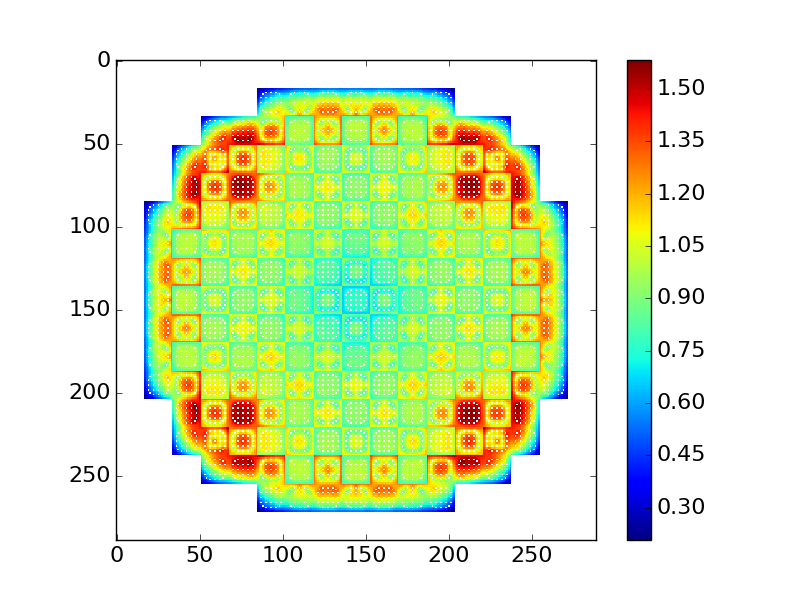
\includegraphics[width=0.8\linewidth]{figures/results/rr-plots/beavrs-3d-radial.png}
	\caption{Radial fission rate distribution for the BEAVRS benchmark formed by OpenMOC with reaction rates axially integrated.}
	\label{fig:full-core-radial}
\end{figure}

\begin{figure}[ht!]
	\centering
	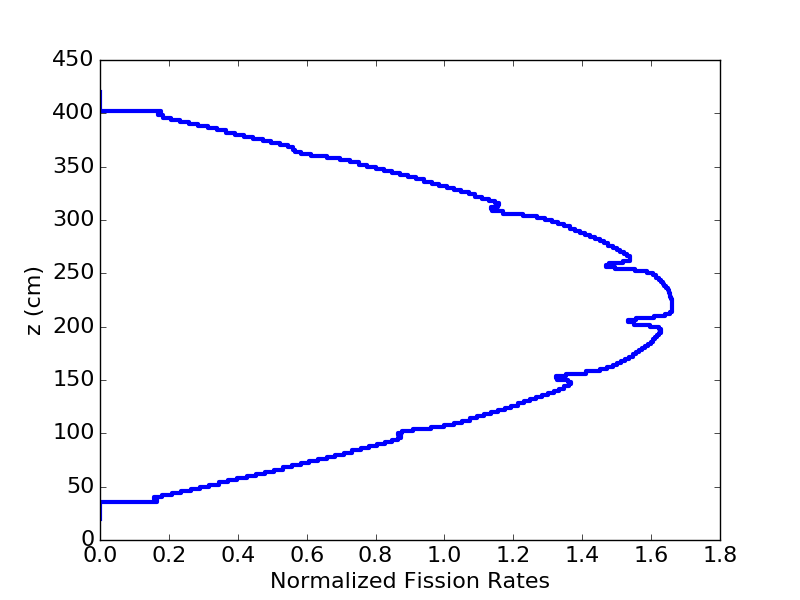
\includegraphics[width=0.8\linewidth]{figures/results/rr-plots/beavrs-3d-axial.png}
	\caption{Axial fission rate distribution for the BEAVRS benchmark formed by OpenMOC with reaction rates radially integrated.}
	\label{fig:full-core-axial}
\end{figure}

\newpage
The OpenMOC results are compared with the OpenMC Monte Carlo solution from which the multi-group cross-sections were derived. The Monte Carlo simulation used 400 batches (300 inactive, 100 active) with $2 \times 10^8$ particles per batch. A comparison of the OpenMOC and OpenMC solutions is presented in Table~\ref{tab:openmc-comparison} in which fission rates are calculated on a pellet-wise scale (2.0 cm axial height).

\begin{table}[ht]
	\centering
	\caption{Simulation accuracy of OpenMOC relative to an OpenMC reference solution}
	\medskip
	\begin{tabular}{l|l|c|c|c}
		%\hline
		&                               & Avg. Fission Rate & \ac{RMS} Fission & Max Fission \\
		& $k_{\textit{eff}}$ eigenvalue & Std. Dev.         & Rate Error & Rate Error \\
		\hline
		OpenMC  & 0.99927 +/- $1 \times 10^{-5}$  & 1.82\% & --     & -- \\
		OpenMOC & 0.99677                         & --     & 2.14\% & 7.52\% \\
		\hline
	\end{tabular}
	\label{tab:openmc-comparison}
\end{table}

Notice that since Monte Carlo simulations introduce statistical noise, each pellet-wise Monte Carlo fission rate has an associated standard deviation. The \ac{RMS} pellet-wise fission rate error of OpenMOC is 2.14\% which is close to the average standard deviation in OpenMC tallies. The radial and axial error distributions are presented in Figure~\ref{fig:openmc-comp-rad} and Figure~\ref{fig:openmc-comp-ax}, respectively, showing a radial tilt across the core.

\begin{figure}[ht!]
	\centering
	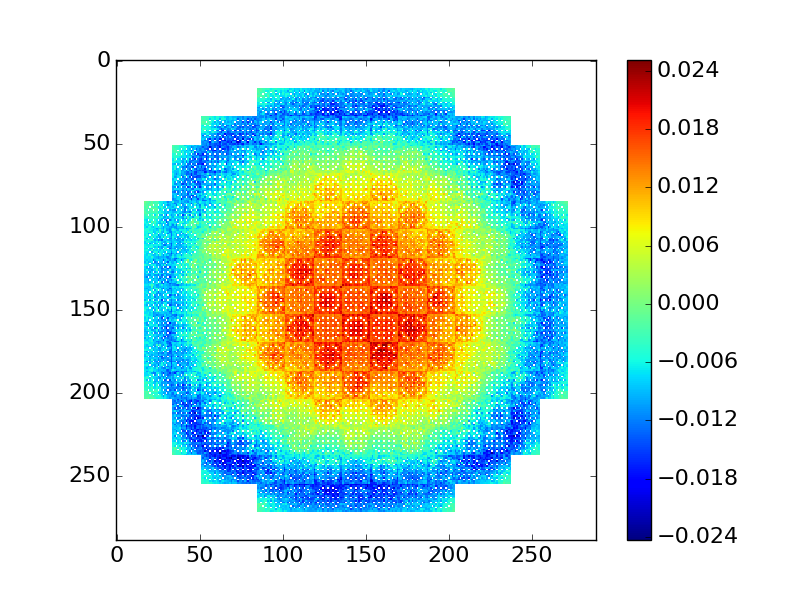
\includegraphics[width=0.6\linewidth]{figures/results/full-core/radial_diff_v_openmc.png}
	\caption{Radial distribution of normalized fission rate errors of OpenMOC compared with a reference OpenMC solution on the BEAVRS benchmark.}
	\label{fig:openmc-comp-rad}
\end{figure}

\begin{figure}[ht!]
	\centering
	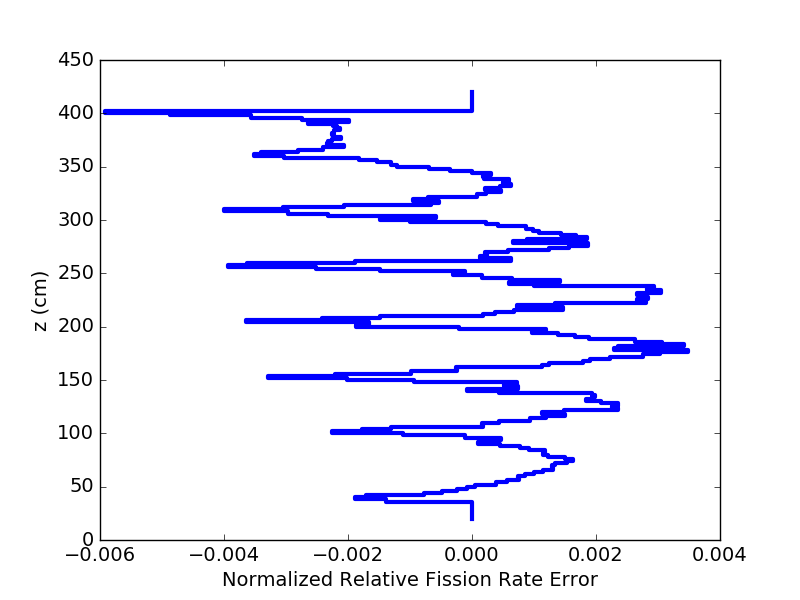
\includegraphics[width=0.6\linewidth]{figures/results/full-core/axial_diff_v_openmc.png}
	\caption{Axial distribution of normalized fission rate errors of OpenMOC compared with a reference OpenMC solution on the BEAVRS benchmark.}
	\label{fig:openmc-comp-ax}
\end{figure}


To ensure the gross fission rate distribution is simulated with reasonable accuracy, assembly-integrated fission rates are compared. Figure~\ref{fig:assembly-rr} shows these assembly rate errors and the associated OpenMC reference folded into a 1/8 map. Similar to the radial distribution shown in Figure~\ref{fig:openmc-comp-rad}, the error again appears as a pure tilt across the core. This tilt is due to the particular transport correction that is not able to fully capture the effects of anisotropic scattering. It is possible that a better transport correction -- particularly in reflector regions -- would be able to eliminate this tilt. However, accurate cross-section formation is not the objective of this thesis and other ongoing projects at MIT are seeking to improve the transport correction.

\begin{figure}[ht!]
	\centering
	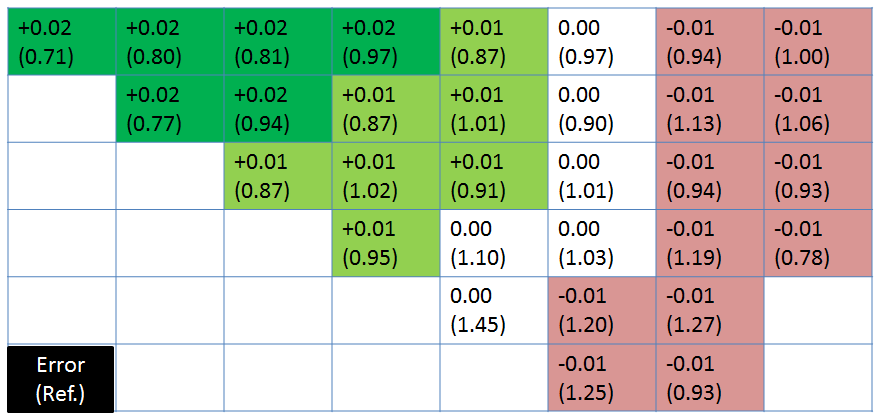
\includegraphics[width=\linewidth]{figures/results/full-core/folded-1-8-core-assembly-rr.png}
	\caption{1/8 core folded assembly fission rate error of OpenMOC compared with the reference OpenMC solution for the BEAVRS benchmark.}
	\label{fig:assembly-rr}
\end{figure}

\section{Computational Performance}
\label{sec:fc-computational-performance}

The computational requirements of the full core solution in OpenMOC is presented in Table~\ref{tab:full-core-comp-req}. Note that while the number of core-hours required to converge the problem is high (717,465), the solution was computed on the Argonne BlueGene/Q supercomputer, which has extremely slow cores for energy efficiency reasons. The requirements on modern computing cores, such as those on the Falcon supercomputer, is estimated by comparing the integration time per core of the SDSA problem tested in Chapter~\ref{chap:linear-source} on the Falcon supercomputer (48.96 ns/core) to those on the Argonne BlueGene/Q supercomputer (175.36 ns/core) for one node using all available cores. However, this case cannot be explicitly simulated due to the small aggregate memory of the Falcon supercomputer.

\begin{table}[ht]
	\centering
	\caption{Computational requirements of OpenMOC on the full core 3D BEAVRS benchmark using the Mira partition of the Argonne BlueGene/Q supercomputer}
	\medskip
	\begin{tabular}{l|l}
		\hline
		Runtime & 7.76 hours \\
		Number of Transport Sweeps & 20 \\
		Nodes & 5780 ($17 \times 17 \times 20$) \\
		CPU Cores & 92480 \\
		Integration Time per Core & 256.7 ns / core \\
		Computational Cost & 717,465 core-hours \\
		Estimated Computational Cost on Falcon & $\approx$ 200,314 core-hours \\
		\hline
	\end{tabular}
	\label{tab:full-core-comp-req}
\end{table}

Further analysis of the computational profile is presented in Table~\ref{tab:full-core-comp-prof}. The results show the computational overhead of CMFD acceleration was insignificant. In addition, the time spent communicating boundary angular fluxes between domains was quite small. However, there was significant idle time between sweeps when nodes are waiting for others to finish their current iteration. This is an indication of load imbalance due to more work being required in core regions than in reflector regions.

\begin{table}[ht]
	\centering
	\caption{Computational profile of OpenMOC on the full core 3D BEAVRS benchmark using the Mira partition of the Argonne BlueGene/Q supercomputer}
	\medskip
	\begin{tabular}{lll|c|c}
		\hline
		& & & Computation & Fraction of \\
		\multicolumn{3}{c|}{Solver Component} & Time (s) & Runtime\\
		\hline
		Total & & & $2.79 \times 10^4$ & 100\% \\
		& Transport Sweeps & & $2.67 \times 10^4$ & 95.8\% \\
		& & Angular Flux Communication & $7.05 \times 10^2$ & 2.5\% \\
		& & Idle Time Between Sweeps & $7.74 \times 10^3$ & 27.7\% \\
		& CMFD Solver & & $97.4$ & 0.3\% \\		
		\hline
	\end{tabular}
	\label{tab:full-core-comp-prof}
\end{table}

\newpage

\section{Comparison with Flat Source MOC}
\label{sec:fc-flat-source}

Using the same \ac{MOC} parameters, the BEAVRS core is simulated using the flat source solver. It is important to note that this case is not expected to be spatially converged since the mesh discretization was derived from linear source \ac{MOC} sensitivity studies. Instead, the purpose is to compare the computational performance of the flat and linear source solvers to understand the overhead of the linear source approximation as well as possible differences in convergence behavior. The results are presented in Table~\ref{tab:fc-comp-flat-linear}, which again shows a factor of two to three overhead for the linear source solver. Also, the flat source solution converges 3 iterations faster than the linear source equivalent. 

\begin{table}[ht]
	\centering
	\caption{Comparison of Flat and Linear source 3D \ac{MOC} solvers on the BEAVRS benchmark with fixed mesh and ray spacing parameters}
	\medskip
	\begin{tabular}{l|l|l}
		\hline
		 & Flat Source & Linear Source \\
		\hline
		%$k_{\textit{eff}}$ & 0.99662 & 0.99677 \\
		%$\Delta k_{\textit{eff}}$ (pcm) & 15 & -- \\
		Iterations & 17 & 20 \\
		Run Time (hours) & 3.13 & 7.76 \\
		Time per Iteration (minutes) & 11.0 & 23.3 \\
		Core-hours & 289,488 & 717,465 \\
		Integration Time per Core (ns) & 116.2 & 256.7 \\
		\hline
	\end{tabular}
	\label{tab:fc-comp-flat-linear}
\end{table}

\section{Parameter Refinement}
\label{sec:fc-parameter-refinement}

In order to verify that the chosen \ac{MOC} parameters where sufficient in accurately converging the solution in space and angle, simulations are conducted in which each 3D parameter is refined, with the results shown in Table~\ref{tab:fc-param-sensitivity}. Ideally, all parameters should be refined together, but the computational burden would be too large to run on Mira. Therefore, each parameter is refined separately. Due to memory constraints, ray parameters were only able to be refined by $\approx 1.5 \times$ but the axial mesh could be refined by a factor of 2. These results indicate that the solution nearly satisfies to the desired criteria of less than 1.0\% pellet-wise \ac{RMS} fission rate error, less than 3.0\% maximum error, and less than 20 pcm bias with respect to finer parameter solutions. In order to strictly adhere to the criteria, the axial mesh would need to be slightly refined.

\begin{table}[ht]
	\centering
	\caption{Differences observed from refining 3D MOC parameters for the BEAVRS benchmark relative to the first solution}
	\medskip
	\begin{tabular}{l|l|l|c|c|c}
		\hline
		Polar  & Axial Ray & Source & $k_{\textit{eff}}$  & \ac{RMS} Fission & Max Fission \\
		Angles & Spacing   & Height & Bias                & Rate Diff. & Rate Diff. \\
		\hline
		10 & 0.75 cm & 2.0 cm & --     & --     & --  \\
		14 & 0.75 cm & 2.0 cm & 2 pcm  & 0.51\% & 1.92\%  \\
		10 & 0.50 cm & 2.0 cm & 5 pcm  & 0.41\% & 1.76\%  \\
		10 & 0.75 cm & 1.0 cm & 13 pcm & 0.28\% & 3.33\%  \\
		\hline
	\end{tabular}
	\label{tab:fc-param-sensitivity}
\end{table}

\section{Conclusion}
\label{sec:fc-conclusion}

In this Chapter, full core simulation results were presented for the BEAVRS benchmark. The results show reasonable agreement with the OpenMC Monte Carlo solution, though a radial tilt does exist over the core, indicating the need for a better transport correction. Parameter refinement studies were conducted on the full core, showing some sensitivity to axial mesh. However, all parameter refinements nearly met the desired sensitivity criteria. The full core solution required 717,465 core-hours on the Argonne BlueGene/Q supercomputer with slow CPU cores. For more modern CPU cores, it is estimated that only $\approx$ 200,314 core-hours would be required, showing that full core 3D \ac{MOC} simulations are now feasible on modern supercomputers.


\vfill
\begin{highlightsbox}[frametitle=Highlights]
\begin{itemize}
  \item Full core simulation of the BEAVRS benchmark in OpenMOC had a pellet-wise fission rate error of 2.14\% relative to the OpenMC reference solution, which is close to the average standard deviation in OpenMC tallies
  
  \item The vast majority of computation time was spent during on-node transport sweeps with very little time spent communicating boundary information
  
  \item 27.7\% of computation time was spent waiting for other nodes to finish local work, indicating a load imbalance, likely due to less source regions in the radial reflector
  
  \item A narrow parameter refinement study on the full core BEAVRS benchmark showed little sensitivity around the parameters expected for spatial and angular convergence
  
  \item The full core solution required 717,465 core-hours on the Argonne BlueGene/Q supercomputer, equivalent to $\approx$ 200,314 core-hours on modern CPU cores
\end{itemize}
\end{highlightsbox}
\vfill
